The breakdown of the implementation section of this paper will break apart every package into a section. Subsequently every single module will be a subsection. At the top of the section will be a brief package definition (what the package does, how it does it) on a high level.
%%%%%%%%%%%%%%%%%%%%%%%%%%%%%%%%%%%%%%%%%%%%%%%%%%%%%%%%%%%%%%%%%%%%%%%%%%%%%%%%
\section{The Database Structure}
%%%%%%%%%%%%%%%%%%%%%%%%%%%%%%%%%%%%%%%%%%%%%%%%%%%%%%%%%%%%%%%%%%%%%%%%%%%%%%%%
The database structure was designed to be as simple and extensible as possible. There are three tables, 'edge', 'node', and 'status'. As you may imagine, the 'edge' table stores all relationships between 'node' objects, the 'node' table stores all nodes, and the 'status' table stores all statuses.
\subsection{ORM \& Design Decisions}
The ORM of choice for this project was SqlAlchemy due to its' highly adaptable nature and clean access to an agnostic SQL backend (you are able to use Sqlite, Postgresql, Mysql... with SqlAlchemy). Unfortunately the nature of SqlAlchemy is that is not a document database, it is a relational database. Other databases such as MongoDB, and Neo4j support graph operations, at the cost of a less clean integration with the Python workflow. Furthermore, MongoDB has been shown to be unreliable, losing records, crashing, etc. For this reason, SQL Alchemy was chosen.
\subsection{The Declarative Base}
The Declarative Base is a special feature of SQLAlchemy. By extending the base class and providing some protected members with metadata, we are able to create a table of a given type in SQLAlchemy. In the example below, we have created a class Node that extends Base. For our metadata we have provided \verb|__tablename__| which indicates what the table name within our database will be. Additionally we have defined all of the fields and their types which will automatically be instantiated by SQLAlchemy when the engine is created. Additionally you'll see that we have a one:many relationship defined between a given Node and a set of Statuses. That is, a Node can have multiple Statuses (this represents all of the tweets made by the user).
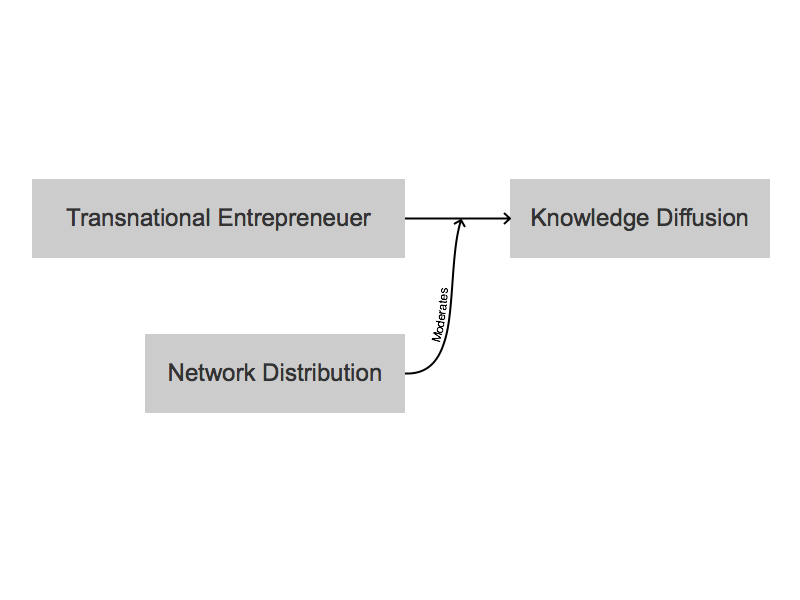
\includegraphics[width=1.0\textwidth]{theoretical_model.png}
